\documentclass[12pt,a4paper]{report}

\usepackage[T1]{fontenc}
\usepackage[utf8]{inputenc}
\usepackage[margin=2.5cm]{geometry}
\usepackage{graphicx}
\usepackage{pdflscape}
\usepackage{tikz}
\usetikzlibrary{arrows.meta,calc,fit,backgrounds}
\usepackage[hidelinks]{hyperref}

% Allow compilation from either the repository root or the report directory.
\makeatletter
\def\input@path{{report/}}
\makeatother

\newcommand{\repo}{https://github.com/womeier/authentikate/blob/main/}
\newcommand{\source}[2]{\href{\repo#1}{#2}}
\newcommand{\code}[1]{\texttt{\detokenize{#1}}}
\newcommand{\ty}[1]{{\footnotesize\ttfamily\detokenize{#1}}}
\newcommand{\links}[2]{\smallskip\source{#1}{Implementation}\quad\source{#2}{Adapter}}
\newcommand{\tested}{\textbf{Tested; no formal proof.}}
\newcommand{\partialproof}{\textbf{Selected source properties proved.}}
\newcommand{\trusted}{\textbf{External capability; assumed.}}

\title{Authentikate Report}
\author{Wolfgang Meier}
\date{\today}

\begin{document}

\maketitle
\tableofcontents

\chapter{Introduction}
Introduce the topic, motivation, and objectives of the report.

\chapter{Background}
Describe the relevant concepts and related work.

\chapter{Implementation}
Explain the approach, design, and implementation.

\section{Architecture}
Figure~\ref{fig:architecture} shows the backend components and verification
boundaries. Figure~\ref{fig:login-flow} traces the login request and its possible
outcomes.

\begin{landscape}
\begin{figure}[p]
\centering
\resizebox{0.85\linewidth}{!}{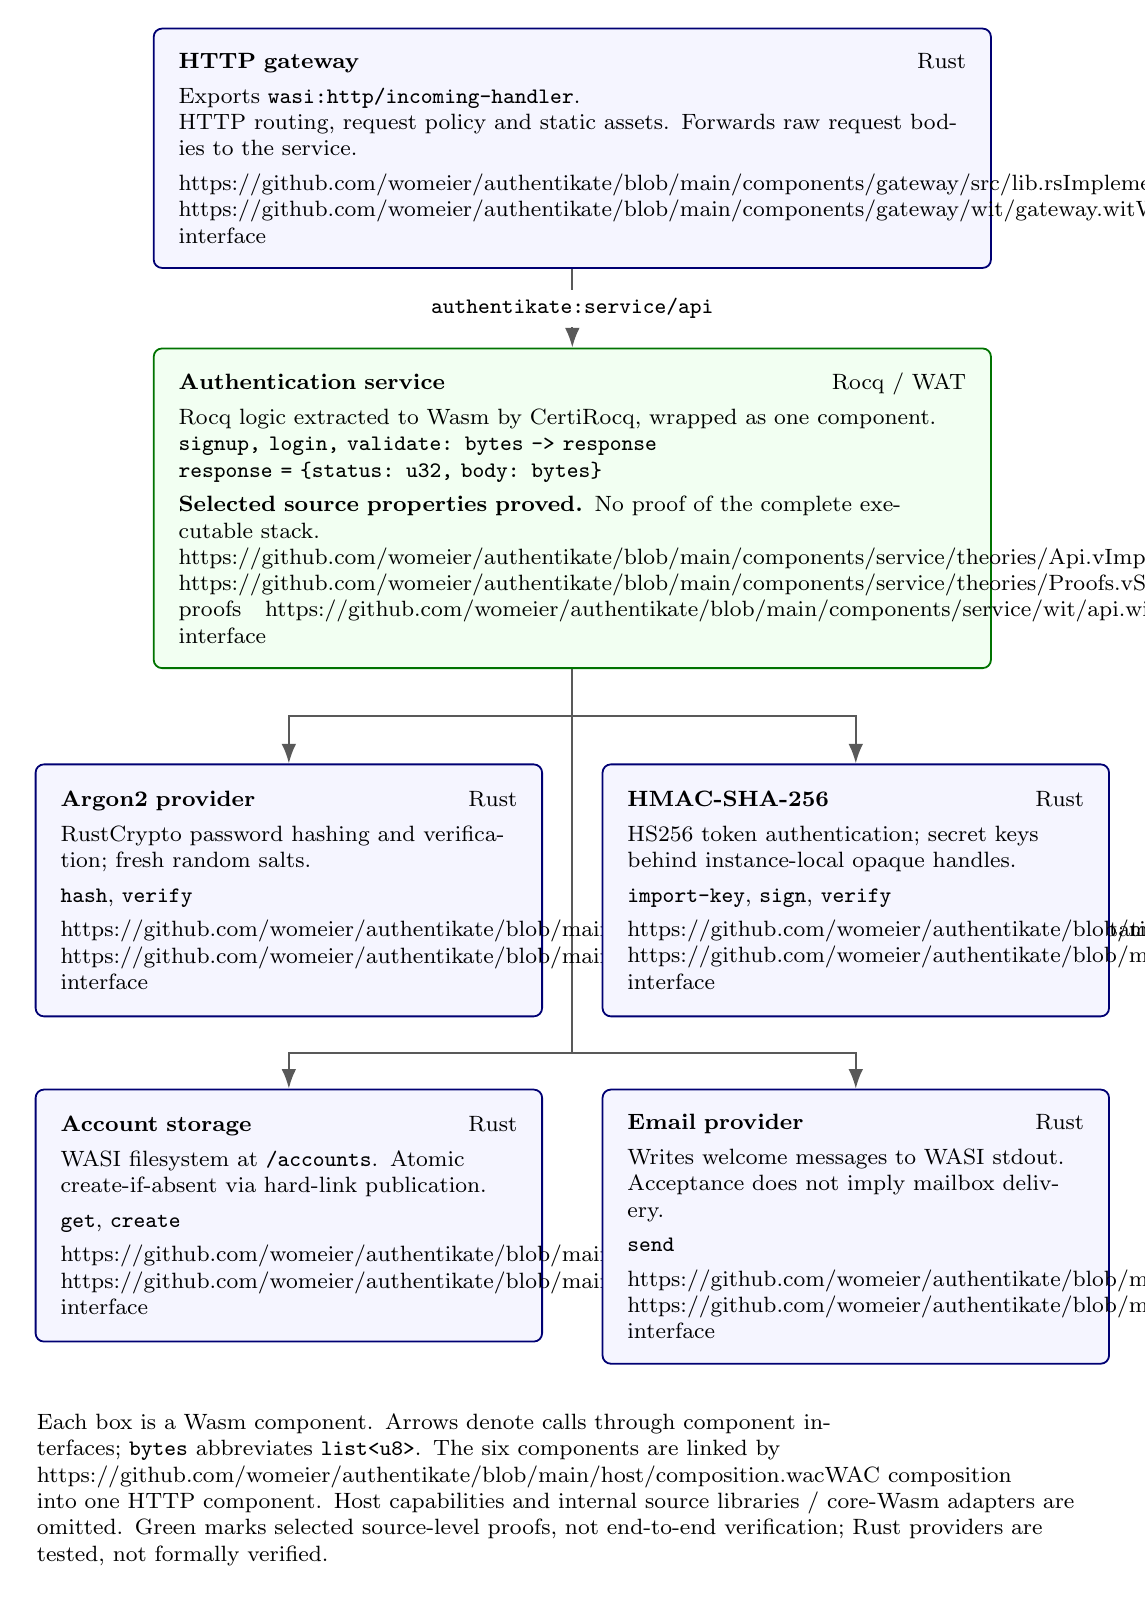
\begin{tikzpicture}[
  x=1cm,y=1cm,
  card/.style={draw=blue!45!black,rounded corners=3pt,line width=.65pt,
    fill=blue!4,text width=5.8cm,minimum height=3.2cm,
    inner sep=9pt,align=left,font=\footnotesize,anchor=north},
  service/.style={card,fill=green!5,draw=green!45!black,text width=10cm},
  flow/.style={-{Latex[length=2.5mm]},line width=.8pt,draw=black!65},
  edge label/.style={font=\footnotesize,fill=white,inner sep=3pt,align=center}
]
\node[card,text width=10cm,minimum height=2.5cm] (gateway) at (0,0) {
  \textbf{HTTP gateway} \hfill Rust\par\smallskip
  Exports \code{wasi:http/incoming-handler}.\par
  HTTP routing, request policy and static assets.
  Forwards raw request bodies to the service.\par\smallskip
  \source{components/gateway/src/lib.rs}{Implementation}\quad
  \source{components/gateway/wit/gateway.wit}{WIT interface}
};

\node[service,minimum height=3.2cm] (service) at ($(gateway.south)+(0,-1)$) {
  \textbf{Authentication service} \hfill Rocq / WAT\par\smallskip
  Rocq logic extracted to Wasm by CertiRocq, wrapped as one component.\par
  \ty{signup, login, validate: bytes -> response}\par
  \ty{response = {status: u32, body: bytes}}\par\smallskip
  \partialproof{} No proof of the complete executable stack.\par
  \source{components/service/theories/Api.v}{Implementation}\quad
  \source{components/service/theories/Proofs.v}{Source proofs}\quad
  \source{components/service/wit/api.wit}{WIT interface}
};

\coordinate (provider-bus) at ($(service.south)+(0,-.6)$);
\node[card] (argon2) at ($(provider-bus)+(-3.6,-.6)$) {
  \textbf{Argon2 provider} \hfill Rust\par\smallskip
  RustCrypto password hashing and verification;
  fresh random salts.\par\smallskip
  \code{hash}, \code{verify}\par\smallskip
  \source{components/crypto/argon2/src/lib.rs}{Implementation}\quad
  \source{components/crypto/wit/argon2.wit}{WIT interface}
};
\node[card] (hmac) at ($(provider-bus)+(3.6,-.6)$) {
  \textbf{HMAC-SHA-256} \hfill Rust\par\smallskip
  HS256 token authentication; secret keys behind instance-local
  opaque handles.\par\smallskip
  \code{import-key}, \code{sign}, \code{verify}\par\smallskip
  \source{components/crypto/hmac/src/lib.rs}{Implementation}\quad
  \source{components/crypto/wit/hmac.wit}{WIT interface}
};
\node[fit=(argon2)(hmac),inner sep=0pt] (crypto-row) {};
\coordinate (storage-bus) at ($(crypto-row.south)+(0,-.45)$);
\node[card] (storage) at ($(storage-bus)+(-3.6,-.45)$) {
  \textbf{Account storage} \hfill Rust\par\smallskip
  WASI filesystem at \code{/accounts}.
  Atomic create-if-absent via hard-link publication.\par\smallskip
  \code{get}, \code{create}\par\smallskip
  \source{components/storage/src/lib.rs}{Implementation}\quad
  \source{wit/accounts.wit}{WIT interface}
};
\node[card] (email) at ($(storage-bus)+(3.6,-.45)$) {
  \textbf{Email provider} \hfill Rust\par\smallskip
  Writes welcome messages to WASI stdout.
  Acceptance does not imply mailbox delivery.\par\smallskip
  \code{send}\par\smallskip
  \source{components/email/src/lib.rs}{Implementation}\quad
  \source{components/email/wit/email.wit}{WIT interface}
};

% Route the lower provider calls through the gap between the cards.
\begin{scope}[on background layer]
  \draw[flow] (gateway.south) --
    node[edge label]{\code{authentikate:service/api}} (service.north);
  \draw[flow] (service.south) -- (provider-bus) -| (argon2.north);
  \draw[flow] (provider-bus) -| (hmac.north);
  \draw[flow] (provider-bus) -- (storage-bus) -| (storage.north);
  \draw[flow] (storage-bus) -| (email.north);
\end{scope}

\node[fit=(storage)(email),inner sep=0pt] (provider-row) {};
\node[anchor=north,text width=13.6cm,font=\footnotesize,align=left]
  at ($(provider-row.south)+(0,-.5)$) {
  Each box is a Wasm component. Arrows denote calls through component
  interfaces; \code{bytes} abbreviates \code{list<u8>}. The six components are
  linked by \source{host/composition.wac}{WAC composition} into one HTTP
  component. Host capabilities and internal source libraries / core-Wasm
  adapters are omitted. Green marks selected source-level proofs, not
  end-to-end verification; Rust providers are tested, not formally verified.
};
\end{tikzpicture}
}
\caption{Backend architecture, component interfaces, and verification boundaries.}
\label{fig:architecture}
\end{figure}

\begin{figure}[p]
\centering
\resizebox{0.85\linewidth}{!}{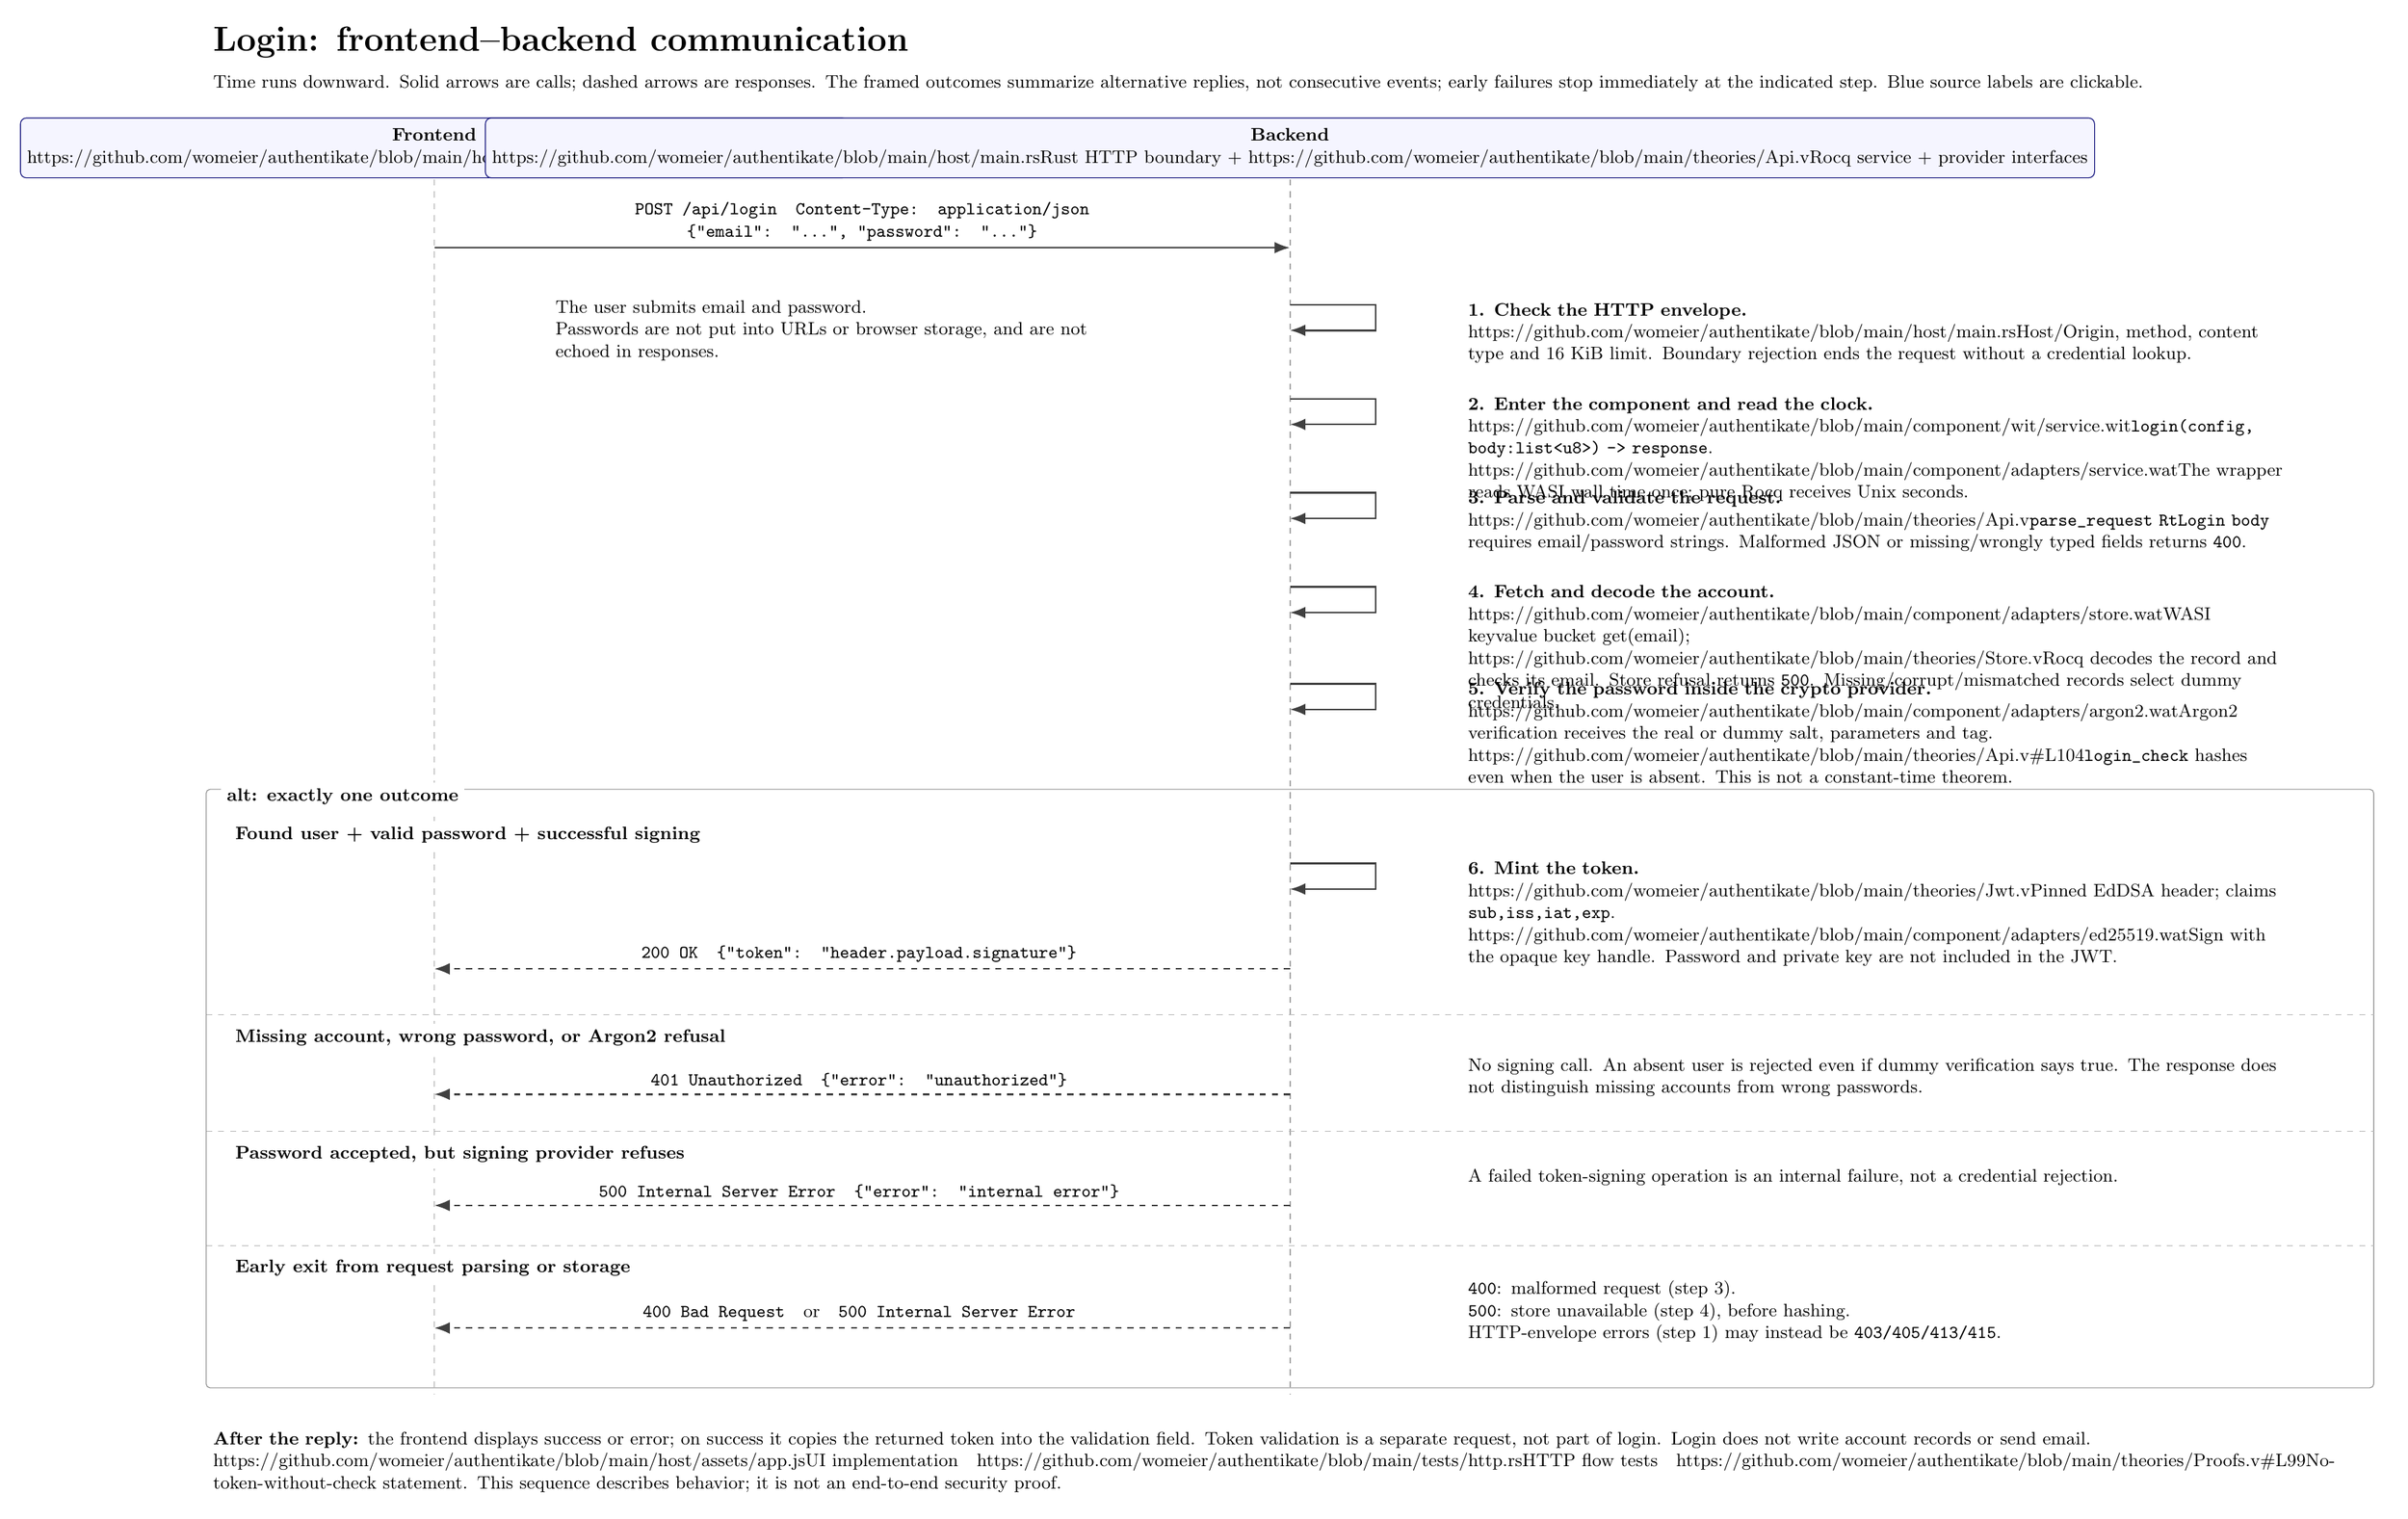
\begin{tikzpicture}[
  x=1cm,y=1cm,
  participant/.style={draw=blue!45!black,fill=blue!4,rounded corners=3pt,
    minimum width=7.8cm,minimum height=1.05cm,align=center,font=\small},
  message/.style={-{Latex[length=2.7mm]},line width=.9pt,draw=black!75},
  reply/.style={message,dashed},
  msglabel/.style={font=\small,fill=white,inner sep=3pt,align=center},
  note/.style={anchor=north west,text width=14.3cm,align=left,font=\small,
    execute at begin node=\raggedright},
  guard/.style={anchor=north west,font=\small\bfseries,fill=white,inner sep=3pt},
  lifeline/.style={draw=black!35,dashed,line width=.7pt}
]
\node[anchor=north west,font=\LARGE\bfseries] at (0,0)
  {Login: frontend--backend communication};
\node[anchor=north west,text width=38cm,font=\small] at (0,-.85)
  {Time runs downward. Solid arrows are calls; dashed arrows are responses.
   The framed outcomes summarize alternative replies, not consecutive events;
   early failures stop immediately at the indicated step. Blue source labels are clickable.};

\node[participant] (frontend) at (4,-2.25) {
  \textbf{Frontend}\\
  \source{host/assets/app.js}{JavaScript UI / fetch client}
};
\node[participant] (backend) at (19,-2.25) {
  \textbf{Backend}\\
  \source{host/main.rs}{Rust HTTP boundary} +
  \source{theories/Api.v}{Rocq service} + provider interfaces
};
\draw[lifeline] (4,-2.8) -- (4,-24.1);
\draw[lifeline] (19,-2.8) -- (19,-24.1);

\draw[message] (4,-4) -- node[msglabel,above] {
  \code{POST /api/login}\quad\code{Content-Type: application/json}\\
  \code{{"email": "...", "password": "..."}}
} (19,-4);
\node[anchor=north west,text width=9.6cm,font=\small,align=left] at (6,-4.8) {
  The user submits email and password.\par
  Passwords are not put into URLs or browser storage, and are not echoed in responses.
};

\draw[message] (19,-5) -- (20.5,-5) -- (20.5,-5.45) -- (19,-5.45);
\node[note] at (22,-4.85) {
  \textbf{1. Check the HTTP envelope.}\par
  \source{host/main.rs}{Host/Origin, method, content type and 16 KiB limit}.
  Boundary rejection ends the request without a credential lookup.
};

\draw[message] (19,-6.65) -- (20.5,-6.65) -- (20.5,-7.1) -- (19,-7.1);
\node[note] at (22,-6.5) {
  \textbf{2. Enter the component and read the clock.}\par
  \source{component/wit/service.wit}{\code{login(config, body:list<u8>) -> response}}.
  \source{component/adapters/service.wat}{The wrapper reads WASI wall time once}; pure Rocq receives Unix seconds.
};

\draw[message] (19,-8.3) -- (20.5,-8.3) -- (20.5,-8.75) -- (19,-8.75);
\node[note] at (22,-8.15) {
  \textbf{3. Parse and validate the request.}\par
  \source{theories/Api.v}{\code{parse_request RtLogin body}} requires email/password strings.
  Malformed JSON or missing/wrongly typed fields returns \code{400}.
};

\draw[message] (19,-9.95) -- (20.5,-9.95) -- (20.5,-10.4) -- (19,-10.4);
\node[note] at (22,-9.8) {
  \textbf{4. Fetch and decode the account.}\par
  \source{component/adapters/store.wat}{WASI keyvalue bucket get(email)};
  \source{theories/Store.v}{Rocq decodes the record and checks its email}.
  Store refusal returns \code{500}. Missing/corrupt/mismatched records select dummy credentials.
};

\draw[message] (19,-11.65) -- (20.5,-11.65) -- (20.5,-12.1) -- (19,-12.1);
\node[note] at (22,-11.5) {
  \textbf{5. Verify the password inside the crypto provider.}\par
  \source{component/adapters/argon2.wat}{Argon2 verification} receives the real or dummy salt, parameters and tag.
  \source{theories/Api.v\#L104}{\code{login_check}} hashes even when the user is absent.
  This is not a constant-time theorem.
};

% Mutually exclusive replies. Early exits refer back to the numbered steps.
\draw[draw=black!45,rounded corners=2pt] (0,-13.5) rectangle (38,-24);
\node[guard] at (.25,-13.38) {alt: exactly one outcome};
\node[guard] at (.4,-14.05) {Found user + valid password + successful signing};

\draw[message] (19,-14.8) -- (20.5,-14.8) -- (20.5,-15.25) -- (19,-15.25);
\node[note] at (22,-14.65) {
  \textbf{6. Mint the token.}\par
  \source{theories/Jwt.v}{Pinned EdDSA header; claims \code{sub,iss,iat,exp}}.
  \source{component/adapters/ed25519.wat}{Sign with the opaque key handle}.
  Password and private key are not included in the JWT.
};
\draw[reply] (19,-16.65) -- node[msglabel,above] {
  \code{200 OK}\quad\code{{"token": "header.payload.signature"}}
} (4,-16.65);

\draw[draw=black!30,dashed] (0,-17.45) -- (38,-17.45);
\node[guard] at (.4,-17.6) {Missing account, wrong password, or Argon2 refusal};
\draw[reply] (19,-18.85) -- node[msglabel,above] {
  \code{401 Unauthorized}\quad\code{{"error": "unauthorized"}}
} (4,-18.85);
\node[note] at (22,-18.1) {
  No signing call. An absent user is rejected even if dummy verification says true.
  The response does not distinguish missing accounts from wrong passwords.
};

\draw[draw=black!30,dashed] (0,-19.5) -- (38,-19.5);
\node[guard] at (.4,-19.65) {Password accepted, but signing provider refuses};
\draw[reply] (19,-20.8) -- node[msglabel,above] {
  \code{500 Internal Server Error}\quad\code{{"error": "internal error"}}
} (4,-20.8);
\node[note] at (22,-20.05) {
  A failed token-signing operation is an internal failure, not a credential rejection.
};

\draw[draw=black!30,dashed] (0,-21.5) -- (38,-21.5);
\node[guard] at (.4,-21.65) {Early exit from request parsing or storage};
\draw[reply] (19,-22.95) -- node[msglabel,above] {
  \code{400 Bad Request}\quad or\quad\code{500 Internal Server Error}
} (4,-22.95);
\node[note] at (22,-22) {
  \code{400}: malformed request (step 3).\par
  \code{500}: store unavailable (step 4), before hashing.\par
  HTTP-envelope errors (step 1) may instead be \code{403/405/413/415}.
};

\node[anchor=north west,text width=38cm,font=\small] at (0,-24.65) {
  \textbf{After the reply:} the frontend displays success or error; on success it
  copies the returned token into the validation field. Token validation is a
  separate request, not part of login. Login does not write account records or
  send email. \source{host/assets/app.js}{UI implementation}\quad
  \source{tests/http.rs}{HTTP flow tests}\quad
  \source{theories/Proofs.v\#L99}{No-token-without-check statement}.
  This sequence describes behavior; it is not an end-to-end security proof.
};
\end{tikzpicture}
}
\caption{Frontend--backend login flow and alternative responses.}
\label{fig:login-flow}
\end{figure}
\end{landscape}

\chapter{Conclusion}
Summarize the results and discuss future work.

\end{document}
